
\begingroup % redefine this macro for this chapter
\def\mult(#1){\operatorname{mulsec}#1} % NB \index{mulsec|defi} occurs below

\chapter[Hyperplane sections of a curve]{Hyperplane sections\\of a curve}
\label{linear general position chapter}

One way to study a curve in $\PP^r$ is to use properties of its hyperplane
sections. In this chapter, we will take up the question: if $C \subset
\PP^r$ is a reduced, irreducible and nondegenerate curve, what can we say
about the geometry of the points in the  hyperplane section
$\Gamma = C \cap H$ of $C$, and what more can we say about a general hyperplane
section?

We prove and apply a result originally due to Castelnuovo,
\index{Castelnuovo @Castelnuovo, Guido}%
that every subset of $r$ points in a
general hyperplane section
\index{general hyperplane section}%
of $C$ spans the hyperplane; that is, any $r$
points of $\Gamma$ are linearly independent.
Recall (from just above Proposition \ref{points on rnc}) that
in this situation
the points
are said to be
in \emph{linearly general position}.
\index{linearly general position}%
Castelnuovo's result
holds for smooth curves in
any characteristic;
\index{positive characteristic}%
Exercise \ref{strange curves} has
counterexamples involving singular curves in positive
characteristic.

This is followed by a series of applications,
including
a
\index{Castelnuovo's theorem}%
famous theorem of Castelnuovo bounding the genus of a
curve in terms of its degree,
and, through that result, a proof that canonical curves and linearly
normal curves ``of high degree'' are arithmetically Cohen--Macaulay
\index{ACM}%
(Theorem~\ref{list of Castelnuovo curves}).

In Chapter~\ref{uniform position}, we will explain and prove a still
stronger general position result, which requires characteristic 0, and
give applications to the irreducibility of fiber products, to the Hilbert
functions of subsets of the
general hyperplane section, and to sums of linear series.

\section{Linearly general position}\label{linearly general position
section}
In this section we
allow our algebraically closed ground field to
have arbitrary characteristic.

An irreducible and reduced curve
$C\subset \PP^r$ over an algebraically closed field,
other than a
\index{strange curve|defi}%
line, is called \emph{strange} if
all the tangent lines at smooth points of $C$ meet in a point $p\in \PP^r``$.
If this condition seems somewhat\dots\ strange, that may be because no
such curves exist in characteristic 0: if
all the
tangent lines at smooth points of $C$ met in a point, then the projection
of $C$ from that point would have derivative 0 everywhere and hence be
constant. But strange curves do exist in
positive
characteristic, albeit
\index{Samuel @Samuel, Pierre}%
rarely: Pierre Samuel showed that the only \emph{smooth} curve that is
strange (in any characteristic) is the conic in
characteristic 2;
a proof
is given in \cite[Theorem IV.3.9]{Hartshorne1977}. Without the smoothness
hypothesis there are more examples; see Exercise~\ref{strange curves}.



\begin{npt}
\begin{theorem}[{{\cite[Lemma 1.1]{Rathmann}}}]
\label{basic linear independence}\label{linear general position}
\index{Rathmann, J\"{u}rgen}%
Suppose that $n\geq 3$. If $C\subset \PP^r$ is a nondegenerate,
irreducible, reduced curve
that is not strange,
and $H$ is a general hyperplane, then any $r$ points of $H\cap C$ are
linearly independent.
\unif
\end{theorem}
\end{npt}

We postpone the proof to introduce some related definitions.

For example, the theorem says that for $C \subset \PP^3` `$, the general
hyperplane section does not contain a line
\index{multisecant}%
that meets $C$ three or more times\emdash a \emph{multisecant}. Another
special configuration which is not present in a general hyperplane
section, as it turns out,
is any pair of points $p\neq q$ on $C$ such that the tangent lines
to $C$ at $p$ and $q$ intersect\emdash what was
classically
\index{stationary secant}%
called a
\textit{stationary secant}
(Figure~\ref{Fig9.1}).

\begin{figure}
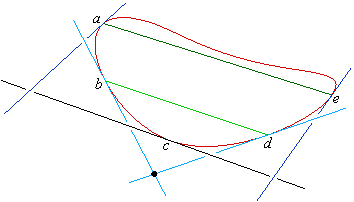
\includegraphics[height=1.5in]{main/cradle-good}
\caption{The lines $bd$ and $ae$ are stationary secants to a degree
  four space curve in red, because the tangents at $b$ and $d$
  have a nonempty intersection, as do (at infinity) the tangents at
  $a$ and $e$.}
\label{Fig9.1}
\end{figure}

More formally we define two subsets of the symmetric square $C_2$ of $C$:
\index{mulsec|defi}%
\index{stat|defi}%
$$
\begin{aligned}
 \mult(C) &\colonequals \{@(p,q) \in C_2 \mid \overlw20{pq} \hbox{ meets
 $C$ in a scheme of length $\geq 3$}@\},\\
\stat(C) &\colonequals  \{@(p,q) \in C_2\setminus \Delta \mid  \hbox{the
tangent lines to $C$ at $p,q$ meet}
@\}.
\end{aligned}
$$
Here
$\overlw20{pq}$
denotes the secant line through $p,q$ (or the
tangent line if $p=q$) and $\Delta\subset C_2$
is the diagonal.


Clearly if $C$ is strange or planar then $\stat(C) = C_2\setminus \Delta$,
and
if $C$ is
planar with $\deg C>2$ then $\mult(C) = C_2$.
These are the only such cases:

\begin{proposition}\label{mult and stat}
 If $C\subset \PP^r$ is a reduced, irreducible, curve that is neither
 planar nor strange, then $\mult(C)\subset C_2$
 and $\stat(C)\subset C_2\setminus \Delta$ are closed subsets of dimension
at most
 $1$.
\unif
\end{proposition}

\begin{proof}
To show that $\mult(C)$ is closed, consider the projection map
$$
\{((p,q), r) \in C_2\times \PP^r \mid r \in \overlw20{pq}@\} \to C_2
$$
sending  $((p,q),r)$ to $(p,q)$. By the
semicontinuity of the degree
\index{semicontinuity!of degree}%
in proper families of constant fiber dimension, the set of points lying
in fibers
of length $\geq 3$ is closed, and $\mult(C)$ is the image of this
set. Because the map is finite,
$\mult(C)$  is closed as well.

Similarly, since
$
\{((p,q), r) \in (C_2\setminus \Delta)\times \PP^r \mid r \in {\mathbb T}_p(C)\cup
{\mathbb T}_q(C) \}
$
is closed in $(C_2\setminus \Delta)\times \PP^r` `$, its image under
the projection to the first factor,
which is $\stat(C)$, is closed in $C_2\setminus \Delta$.

Suppose, contrary to the proposition, that $\dim \stat(C) >1$. Since
$\stat(C)$ is a closed subset of the irreducible variety $C_2\setminus
\Delta$ it
follows that $\stat(C) = C_2\setminus \Delta$, so every pair of tangent
lines meet. Any three
lines in projective space that meet pairwise must be either coplanar or
meet in a point. Thus if $C$ is not strange,
then all the tangents to $C$ lie in a common plane, and $C$ is planar,
contradicting our hypothesis
and proving that $\dim \stat(C)\leq 1$.

Finally suppose, contrary to the proposition,  that $\dim \mult(C)>1$. As
in the previous argument, this
implies that every secant is a multisecant.  We will show in this case
that $\dim \stat(C) =2$, a contradiction.

To this end, consider the projections $\pi_{p}: C \to \PP^{r-1}$ and
the set
$$
\tabcolsep1pt
I = \Bigl\{(p,r,r') \in C^3 \Bigm|
\begin{tabular}{l}\small $p,r,r'$ are distinct and\\[-2pt]
\small $\pi_{p}(r) = \pi_{p}(r')$ is a smooth point of $\pi_p(C)$
\end{tabular}
\Bigr\}.
$$
The tangent lines ${\mathbb T}_r(C)$ and ${\mathbb T}_{r'}(C)$ both project from $p$ to the
tangent line ${\mathbb T}_{\pi_p(r)}(\pi_C)$,
and thus they lie in the 2-plane spanned by $p$ and this line; it follows
that $(r,r') \in \stat(C)$.
The projection $I \to C_2: (p,r,r') \mapsto (r,r')$ is finite since the
secant line $\overkern10{rr'}$ meets $C$ in only finitely many points,
so $\dim I \leq \dim \stat(C)$.

 If the projection from some point $p$ were everywhere ramified,
then all tangents to $C$ would pass through $p$, and $C$ would be strange.
Since also every secant to $C$ is a multisecant it follows that  for
every smooth point $p\in C$ there is an open set of points $q\in \pi_p(C)$
such that
the fiber $\pi_p^{-1}(q)$ contains two distinct points of $C$. Thus the
projection $I \to C: (p,r,r') \mapsto p$ maps
$I$ onto an open set of $C$, with 1-dimensional fibers, so $2 = \dim
I\leq \dim \stat(C)$ as claimed.
\end{proof}


\begin{proof}[Proof of Theorem~\ref{linear general position}]
If
$C\subset \PP^n$ is a reduced curve then, by Bertini's theorem, a general
\index{Bertini's theorem}%
hyperplane meets $C$ transversely.
First suppose that $n=3$, and consider the incidence correspondence
$$
I \colonequals  \{ ((p,q), H) \in \mult(C) \times (\PP^3)^* \mid
\overlw20{pq}\in H\}.
$$
Since $\dim \overlw20{pq} = 1$, the fibers of the projection of $I$
to $\mult(C)$ have dimension 1,
so $\dim I = 1+\dim \mult(C)  \leq 2$. Consequently the image of  the
projection of $I$ to $(\PP^3)^*$ has
dimension $\leq 2$, so there is an open set of planes that contain no
multisecants, proving the theorem in this case.

\begin{fact}
 Since a secant line to a curve $C$ that is not itself a line is
 determined by its intersections with $C$,
 every curve other than a line has a 2-parameter family of secant
 lines. If $C\subset \PP^3$ is nondegenerate,
 this means that it is 2 conditions for a line in $\PP^3$ to be a secant
 to $C$. Since a pencil of lines meets
 $C$ in codimension 1, one might expect that, correspondingly, there
 would be a 1-parameter family
 of trisecant lines and a finite number of 4-secant lines. One can
 compute the expected number enumeratively
 \cite[p.~296]{Griffiths-Harris1978}.
 For example a general curve of degree $\leq 4$ can have no 4-secant
 line (it would meet planes containing that line in at least 5 points),
 but a general rational curve of degree 5 in $\PP^3$
  has exactly 1 \cite[Section 12.4.4]{3264}. See  Figure~\ref{9.2}
  for a construction in which the 4-secant line is visible.

\begin{figure}[b]
\centerline {\includegraphics[height=1.5in]{"main/Fig09-2"}}
\caption{A smooth rational quintic in $\PP^{3}$ with a unique 4-fold
secant line
can be obtained as the image of a plane conic $C$ by the rational map
of $\PP^{2}$ to $\PP^{3}$
induced by the 4 cubics through 6 points $e_{1},\dots e_{6}$, exactly
one of which lies on $C$; the image of the unique conic $D$ through the
other 5 points becomes the 4-secant line to the image of $C$.
}
\label{9.2}
\end{figure}

 This fact entered history in a peculiar way:
 After Kronecker \citeyear{Kronecker} proved that every algebraic set in
  $\PP^{n}$ is set-theoretically the intersection of $n+1$
\index{Vahlen @Vahlen, Karl Theodor}%
\index{Kronecker @Kronecker, Leopold}%
\index{set-theoretic equality}%
\index{quintic curve!rational}%
  hypersurfaces,
Vahlen \citeyear{Vahlen} claimed that Kronecker's result was
  sharp ``because'' a general
rational quintic
\index{historical context}%
with one 4-secant line
  could not be the intersection of 3 hypersurfaces.
  Vahlen played a role in the rise of the Nazi party, and perhaps for
  that reason
Perron \citeyear{Perron} produced 3 hypersurfaces intersecting
\index{Perron @Perron, Oskar}%
  precisely in a given general rational quintic. It is now known that
  every algebraic set in
  $\PP^{n}$ over an infinite field can be written set-theoretically as
  the intersection of just $n$ hypersurfaces \cite{Eisenbud-Evans}.
\end{fact}

We next do induction on $n\geq 4$. We will show first that the image
$C'$ of
$C$ under the projection $\pi_p: C\to C'$ from a general point of $C$
is not strange. Since $C\subset \PP^r$ is neither
planar nor strange
Proposition~\ref{mult and stat} shows that we may choose two smooth points
$r,r'\in C\subset \PP^r$ such that ${\mathbb T}_r(C)\cap {\mathbb T}_{r'}(C) = \emptyset$,
and thus
${\mathbb T}_r(C)$ and ${\mathbb T}_{r'}(C)$ together span a 3-plane $L$. Since $C$ is
nondegenerate we may
choose a point $p\in C$ outside $L$, and it follows that $\pi_p$
restricted to $L$ is an isomorphism.
Thus ${\mathbb T}_{\pi_p(r)}(C') \cap {\mathbb T}_{\pi_p({r'})}(C') = \emptyset$, so $C'$
is not strange,
and since $n\geq 4$ the curve $C'$ is not planar either.

Arguing by contradiction, suppose that the general hyperplane section
of~$C$ contains a set of $r$ linearly dependent points. Consider the
closed subsets
$$
I_1 \subset I \subset \{@(p,H) \in C \times (\PP^n)^*@\}
,
$$
where $I$ is defined by the
condition
that $p\in H$ and $I_1$ is defined
by the condition that, in addition, there exist $p_2,\dots, p_r\in H$
such that $p, p_2, \dots, p_r$ are dependent. Both $I_1$ and $I$ are
closed subsets.

By hypothesis, both $I_1$ and $I$ project onto open sets of $(\PP^n)^*$,
so they have the same dimension.
But $I$ is irreducible: it projects onto an open subset of $C$ with
fibers isomorphic to $\PP^{r-1}$. Thus $I_1 = I$,
and  $p$ is part of a dependent set
$\{p, p_2,\dots, p_r\}$ in a general hyperplane containing $p$.

Let $H'$ be a general hyperplane in $\PP^{n-1}$
and let $H = \pi_p^{-1}(H')$, which is a general hyperplane containing
$p$. The intersection $H\cap C$
contains $r$ dependent points $\{p, p_2,\dots, p_r\}$, and it follows
that $\pi_p(p_2),\dots,\pi_p(p_n)$
are dependent points of $H'\cap C'$. This contradicts the induction
hypothesis, and proves that
the general hyperplane section of $C$ is in linearly general position.
\end{proof}

 \section{Castelnuovo's theorem}\label{CastelnuovoSection}

Clifford's theorem gives a complete and sharp answer to the question,
\index{Castelnuovo's theorem}%
``what linear series can exist on a curve of genus $g$?''
But maybe that wasn't the question we meant to ask! After all, we're
interested in describing curves in projective space as images of abstract
curves $C$ under maps given by linear series on $C$. Observing that
the linear series that achieve equality in
Clifford's theorem
\index{Clifford's theorem}%
give maps of degree 2 onto a rational curve,
 we might hope that we
would have a
 different and more relevant
answer if we
restrict our attention to linear series $\cD = (\cL,V)$ for which the
\index{birational}%
associated map $\phi_\cD$ is at least  birational onto its image.

A classical result of Castelnuovo does exactly that: it gives a sharp
bound on the
arithmetic genus
\index{arithmetic genus}%
of a reduced, irreducible, nondegenerate
curve of degree $d$ in $\PP^r` `$. To state it, for positive integers $d$
and $r$, let
\index{M@$M=M(d,r)$|defi}%
\label{def of M}
$$
 M \colonequals
M(d,r)
\colonequals
\biggl\lfloor\mfrac{d-1}{r-1}\biggr\rfloor,
$$
so that
$$
 d -1 = M(r-1) + \epsilon
$$
for some $\epsilon =
\epsilon(d,r)
$
 with $0 \leq \epsilon \leq r-2$.
\index{epsilon@$\epsilon=\epsilon(d,r)$|defi}%

\begin{theorem}[Castelnuovo bound]\label{Castelnuovo's bound}
Let $C \subset \PP^r$ be a reduced, irreducible, nondegenerate curve of
\index{Castelnuovo bound}%
degree $d$. With $M$ and $\epsilon$ defined
as above,
$$
p_a(C) \leq \pi(d,r) \colonequals  \frac{M(M-1)}{2}(r-1) + M\epsilon.
$$
Moreover, if $p_a(C) = \pi(d,r)$  then $C$ is arithmetically
\index{ACM}%
Cohen--Macaulay and every hyperplane
section $H\cap C$ has
Hilbert function
\index{Hilbert function}%
$
\dim (R_{H\cap C})_{m} = \min\{m(r-1), d\}.
$
\end{theorem}

We will say that a curve achieving the bound is a \emph{Castelnuovo
\index{Castelnuovo curve}%
curve}.

\subsection*{Proof of Castelnuovo's bound}

The idea of Castelnuovo's proof is simple and beautiful. To start
with, the hypothesis that $C$ is nondegenerate in $\PP^r$ says that
$h^0(\cO_C(1)) \geq r+1$. We'd like to use this and the Riemann--Roch
formula, in the form
$$
g = d+1 - h^0(\cO_C(1)) + h^1(\cO_C(1)),
$$
but this doesn't work because we have a priori no way to estimate
$h^1(\cO_C(1))$.

Castelnuovo's solution  is to derive lower bounds not just on
$h^0(\cO_C(1))$ but on $h^0(\cO_C(m))$ for all $m$; since we know that
$h^1(\cO_C(m)) = 0$ for large $m$, a lower bound on $h^0(\cO_C(m))$
for large $m$ will translate directly into an upper bound on~$g$.

How can we go about estimating $h^0(\cO_C(m))$? The answer is to
derive lower bounds on the successive differences $h^0(\cO_C(m)) -
h^0(\cO_C(m-1))$, by letting $\Gamma = C \cap H$ be a general hyperplane
section of $C$, and viewing $H^0(\cO_C(m-1))$ as the subspace of
$H^0(\cO_C(m))$ consisting of sections vanishing on $\Gamma$. The
estimates we get may seem crude\emdash not surprisingly, considering
how little we know about~$\Gamma$\emdash but remarkably, the bound we
ultimately derive on the genus of $C$ turns out to be sharp!

For the proof, the following definition will be convenient:

\begin{definition}
If $\sV = (V,\cL)$ is a linear series on a variety $X$ and $\Gamma$
\label{indep}
is a subscheme then the \emph{number of conditions imposed by $\Gamma$
on $\sV$} (that is, the number of
independent linear conditions
%\index{independent conditions!linear}%
\index{independent conditions|defi}%
for a
section in $V$ to vanish
identically on $\Gamma$) is the dimension of the image of $V$ in
$H^0(\sL|_\Gamma) = H^0(\sL \otimes \sO_\Gamma)$; or, numerically,
$$
\dim V - \dim \left(V \cap H^0(\cL\otimes \cI_{\Gamma/X}) \right).
$$
\end{definition}

Thus, for example, if $\Gamma \subset \PP^r` `$, then the number of
conditions imposed by $\Gamma$ on $H^0(\cO_{\PP^r}(m))$ is the value
$h_\Gamma(m)$ of the Hilbert function of $\Gamma$ at $m$.
Note that in case $\Gamma$ is zero-dimensional, the number of conditions
imposed by $\Gamma$ on a linear series $V$ is necessarily less than or
equal to the degree $d$ of $\Gamma$; if it is equal we say that $\Gamma$
\emph{imposes independent conditions on $V$}.

\begin{proof}[Proof of Theorem~\ref{Castelnuovo's bound}]
Suppose that $C \subset \PP^r$ is an irreducible, nondegenerate curve. For
large $m$ we have
$h^{0}(\sO_{C}(m)) = md-p_{a}(C) +1$, so to bound the genus from above
we must
bound $h^{0}(\sO_{C}(m))$ from below.

Let $\Gamma = C@\cap@H$ be a general hyperplane section of $C$, and
let $V_m`\subset`H^0(\cO_C(m))$ be the linear series cut on $C$ by
hypersurfaces of degree $m$ in $\PP^r` `$, that is, the image of the
restriction map
$$
H^0(\cO_{\PP^r}(m)) \to H^0(\cO_C(m)).
$$
The number of  conditions imposed by $\Gamma$ on $V_m$ is the rank of
the restriction map
$\rho_m: V_m \to \sO_\Gamma(m)$.
 The number of conditions imposed by $\Gamma$ on $H^{0}(\sO_{C}(m))$
 is the
 rank of the restriction map from this potentially larger space, and
 thus is at least as large. This
 accounts for the inequality in the following:
{\advance\jot-2pt
\begin{align*}
h^0(\cO_C(m)) - h^0(\cO_C(m-1)) & = \text{\# of conditions imposed by
$\Gamma$ on $H^0(\cO_C(m))$}\\
&\geq \text{\# of conditions imposed by $\Gamma$ on $V_m$} \\
&= \text{\# of conditions imposed by $\Gamma$ on $H^0(\cO_{\PP^r}(m))$} \\
&= h_\Gamma(m).
\end{align*}}%
Replacing $m$ by $k$ in the display above and summing
over $k$, we obtain the lower bound
$$
h^0(\cO_C(m)) \geq \sum_{k=0}^m h_\Gamma(k).
$$

In order to bound the genus $C$ from above, we will bound the Hilbert
function of its hyperplane section $\Gamma$  from below; and for this,
we need to know something about the geometry of $\Gamma$. In fact, all
we need to know is Theorem~\ref{linear general position}, which says
that the points of $\Gamma$ are in
linearly general position!
\index{linearly general position}%

\begin{proposition}\label{min hilb}
If $\Gamma \subset \PP^r$ is a collection of $d$ points in linearly
general position that span $\PP^r` `$, then
$$
h_\Gamma(m) \geq
@
\begin{tcases}
mr+1&\hbox{ if $m\leq M(d,r+1)$,}\\
\hfil d &\hbox{ otherwise.}
\end{tcases}
$$
\end{proposition}

One way to understand the bound $mr+1$ is to realize that if $\Gamma$
is any finite subscheme of a rational normal curve $C\subset\PP^r$
of degree $r$,
then $h_\Gamma(m) = \min\{\deg \Gamma,@ mr`+`1\}$ for every $m$
(Exercise~\ref{linear bound is sharp}).
  Thus the bound in Proposition~\ref{min hilb} is best possible.
On the other hand, sets of points on a rational normal curve are almost
the only sets for which the bound is sharp. See Figure~\ref{Fig9.3}
for an illustration.

\begin{figure}
\centerline {\includegraphics[height=1.5in]{"main/Fig09-3"}}
\caption{The case $d = 3\cdot 2+1$: the point $e_{7}$ imposes an additional
condition on the cubics (such as the union of the three lines shown)
passing through
$e_{1},\dots, e_{6}$.}
\label{Fig9.3}
\end{figure}

\begin{proof}
Suppose first that $d \geq mr+1$, and let $p_1,\dots,p_{mr+1} \in
\Gamma$ be any subset of $mr+1$ points. It suffices to show that
$\Gamma' = \{p_1,\dots,p_{mr+1}\}$ imposes independent conditions
on
$H^0(\cO_{\PP^r}(m))$, that is, for any $p_i \in \Gamma'$ there is a
hypersurface $X \subset \PP^r$ of degree $m$ containing all the points
$p_1,\dots, \hat{p_i},\dots,p_{mr+1}$ but not containing~$p_i$.

To construct such an $X$, group the $mr$ points of $\Gamma' \setminus
\{p_i\}$ into $m$ subsets $\Gamma_k$ of cardinality $r$; each set
$\Gamma_k$ will span a hyperplane $H_k \subset \PP^r` `$, and we can
take $X = H_1 \cup \dots \cup H_m$.

In the case where $d<mr+1$, we add $mr+1-d$ general points; each one
imposes exactly one
additional condition on hypersurfaces of degree $m$.
\end{proof}


To complete the proof of Theorem~\ref{Castelnuovo's bound} we add up the
lower bounds in the proposition. To this end, let $C \subset \PP^r$ be
 an irreducible, nondegenerate curve of degree $d$, and  set
$M= M(d,r) = \bigl\lfloor{\frac{d-1}{r-1}}\bigr\rfloor$
as on page~\pageref{def of M}.
We have
\begin{align*}
h^0(\cO_C(M)) &= \sum_{k=0}^M h^0(\cO_C(k)) - h^0(\cO_C(k-1)) \\
&\geq  \sum_{k=0}^M (k(r-1)+1)
= \frac{M(M+1)}{2}(r-1) + M + 1
,
\end{align*}
and similarly
$$
h^0(\cO_C(M+m)) \geq \frac{M(M+1)}{2}(r-1) + M  + md+ 1
.
$$
For sufficiently large $m$, the line bundle $\cO_C(M+m)$ is nonspecial,
so by the
Riemann--Roch theorem,
\index{Riemann--Roch theorem}%
\begin{align*}
g &= (M+m)d - h^0(\cO_C(M+m)) + 1 \\
&\leq (M+m)d - \left(  \frac{M(M+1)}{2}(r-1) + M + 1 + md \right)+1 \\
& = M\bigl( M(r-1) + 1 + \epsilon \bigr) - \left(  \frac{M(M+1)}{2}(r-1)
+ M  \right) \\
&= \frac{M(M-1)}{2}(r-1) + M\epsilon.
\end{align*}


In the case of equality, to show that $C$ is arithmetically
Cohen--Macaulay we must show that $V_{m} = H^0(\cO_C(m))$ for all $m$.
Consider the diagram
\vspace*{3pt}
$$
\small
\xymatrix{
0\ar[r]& 
H^{0}(\sO_{\PP^{r}}(m-1))\ar[r]\ar[d]^{\mathrm{ surjection}}&
H^{0}(\sO_{\PP^{r}}(m))\ar[r]\ar[d]^{\mathrm{ surjection}}&
H^{0}(\sO_{\Gamma}(m))\ar[d]^{=} \\
0\ar[r]& V_{m-1}\ar[r]\ar[d]^{\mathrm{ injection}}&
V_{m}\ar[r]\ar[d]^{\mathrm{ injection}} &
H^{0}(\sO_{\Gamma}(m))\ar[d]^{=} \\
0\ar[r]& H^{0}(\sO_C(m-1))\ar[r]&H^{0}(\sO_C(m))\ar[r] &H^{0}(\sO_{\Gamma}(m))
\rlap{.}
}
\vspace*{3pt}
$$
The top and bottom rows are left exact. From the left exactness of the
bottom row
it follows that the map $V_{m-1}\to V_{m}$ is an injection. From
the left exactness of the
top row it follows that this map is the kernel of the restriction map
$V_{m} \to H^{0}(\sO_{\Gamma}(m))$.
Thus the middle row is also left exact, and we see that the number of
conditions that
$\Gamma$ imposes on $V_{m}$ is equal to $\dim V_{m}-\dim V_{m-1}$.

From the first part of the proof we have inequalities
$$
\displaylines{
 \text{\# of conditions imposed by $\Gamma$ on $H^{0}(\sO_C(m))$}
\hfill\cr\hfill
\geq
\text{\# of conditions imposed by $\Gamma$ on $V_{m}$},
}
$$
that is,
$$
h^0(\cO_C(m)) - h^0(\cO_C(m-1))\geq \dim V_{m}-\dim V_{m-1}
.
$$
If $g = \pi(d,r)$ then these must both be equalities. Thus
for large $m$ the restriction map
$H^{0}(\sO_{\PP^{r}}(m)) \to H^{0}(\sO_{C}(m))$ is surjective, so
\jot=-5pt % mesh sums; scoped by end of proof
\begin{align*}
\sum_{k=0}^m (h^0(\cO_C(k)) - h^0(\cO_C(k-1))
&= h^0(\cO_C(m)) = \dim V_m \\
&= \sum_{k=0}^m (\dim \Vk - \dim \Vkmi).
\end{align*}
However, for each $k$ we have
$$
\dim \Vk - \dim \Vkmi\geq h^0(\cO_C(k)) - h^0(\cO_C(k-1)),
$$
and thus we must have equality for all $k$, whence  $\dim
\Vk
=h^0(\cO_C(k))$ for all $k$; that is, $C$ is arithmetically
\index{ACM}%
Cohen--Macaulay.

Always supposing that  $p_{a}(C) = \pi(d,r)$, the inequalities in
Proposition~\ref{min hilb}
must be equalities, so for a general hyperplane section $\Gamma = H\cap C$
we have $h_{\Gamma}(m) = \min \{m(r-1)+1, d\}$ for all $m\geq 0$. However,
since
$C$ is arithmetically Cohen--Macaulay, $h_{\Gamma}(m) = h^{0}(\sO_{C}(m))
- h^{0}(\sO_{C}(m-1)) $
for every hyperplane section $\Gamma$, completing the proof.
\end{proof}

 \subsection*{Consequences and special cases}

 First of all,
if
$r=2$ we have $\pi(d,r) = \tbinom{d-1}{2}$,
 so every
plane curve
(smooth or not)
is a Castelnuovo curve.
\index{plane curve!is a Castelnuovo curve}%

 In case $r=3$, we have
 $$
 \pi(d,r) =
 \begin{cases}
 \left(\frac{d-2}{2} \right)^2& \quad \text{if $d$ is even}, \\
\noalign{\vskip3pt}
 \left(\frac{d-1}{2} \right)\left(\frac{d-3}{2} \right)& \quad \text{if
 $d$ is odd},
 \end{cases}
 $$
 which we can recognize as the genus of curves of type $(\unfrac{d}{2},
 \unfrac{d}{2} )$ on a quadric surface in case $d$ is even, and the genus
 of curves of type
 $\bigl(\upnfrac{d{+}1}{2}, \upnfrac{d{-}1}{2} \bigr)$
on a quadric when $d$ is odd. Thus
the Castelnuovo bound is sharp when $r=3$ as well.

Indeed, the Castelnuovo bound is sharp for all $d$ and $r$; we'll
prove this, and describe explicitly the curves that achieve it, in
Chapter~\ref{ScrollsChapter}.


\begin{corollary}\label{list of Castelnuovo curves}
Suppose that $C\subset \PP^r$ is a smooth curve of arithmetic genus
$p_{a}$ and degree $d$ embedded by a complete linear series. The curve
$C$ is  Castelnuovo (and thus arithmetically Cohen--Macaulay) if and
only~if one of the following
conditions
holds:
\begin{enumerate}
\item  $d<2r$ and  $d \geq 2p_a+1$.
\item $d=2r$
and
$C$ is a canonical curve.
\item $r=3$, $d>6$,
and
$C$ is a divisor on a (smooth or singular)
irreducible quadric in the class $mH$ or $mH+L$, where $H$ is the class
of a hyperplane and $L$ is the class of a line.
\item  More generally,  $d>2r$
and
$C$ lies on a rational normal scroll in a certain range of divisor classes
\rm
(Theorem~\ref{Castelnuovo examples}).
\end{enumerate}
\end{corollary}

\begin{fact}
Corollary~\ref{list of Castelnuovo curves} remains true with appropriate
definitions also for reduced irreducible curves. This can be proven
with the techniques developed in Chapters~\ref{LinkageChapter}
and~\ref{ScrollsChapter}.
\end{fact}

\begin{proof}
Simple arithmetic shows that if $d\geq 2p_a+1$  then  $d<2r$ and $p_a=
\pi(d,r)$. Moreover if $p_a= \pi(d,r)$ and $d<2r$,
then indeed $d\geq 2p_a+1$, proving~
(1).

If $d= 2r$ then $\pi(d,r) = r+1$, and Clifford's theorem shows that $C$
is a canonical curve, proving
(2).

Now suppose that $r=3, d>6$ and let $\Gamma$ be a hyperplane
section of $C$. Since $h_{\Gamma}(2) = \min\{2\cdot 2+1,@ d\} = 5$,
$\Gamma$
lies on a conic, and
since $C$ is arithmetically Cohen--Macaulay, $C$ must lie on a quadric.
If $C$ is smooth then arithmetic plus the result of Section~\ref{Div of
quadric} establishes the
claim.
For the more general case (4),
and the case $r>3$, see Theorem~\ref{Castelnuovo examples}
in Chapter~\ref{ScrollsChapter}, where we define rational normal scrolls.
\end{proof}

The most important special case is that of canonical curves:

\begin{corollary}\label{canonical hilbert function}
If $C\subset \PP^{g-1}$ is a canonical curve then the Hilbert function
\index{canonical curve}%
\index{Hilbert function}%
\index{homogeneous coordinate ring}%
of the homogeneous coordinate ring $S_{C}$ of  $C$ depends only on $g$,
and is given by
\smallskip %FMT
$$
\dim({S_{C}})_{n} = h^{0}(\cO_{C}(n)) =
\begin{tcases}
 \hfil 0 & \mbox {if } @d<0,\\
 \hfil 1 & \mbox {if } @d=0,\\
 \hfil g & \mbox {if } @d=1,\\
 @(2g{-}2)n + 1 - g & \mbox {if } @d>1.\\
\end{tcases}
$$
\end{corollary}

\begin{proof}
Theorem~\ref{Castelnuovo's bound} implies that the homogeneous coordinate
ring of $C$ can be identified with $\bigoplus_{n\in \ZZ}\HH^0(\sO_C(n))$,
and the dimensions of these spaces are determined by the Riemann--Roch
theorem.
\end{proof}


\begin{fact}
A famous theorem of Gruson and Peskine \citeyear{MR0690647} (see
\index{Gruson @Gruson, Laurent}%
\index{Peskine @Peskine, Christian}%
\cite{MR0689536} for an exposition and also the case of
positive
characteristic) completes the picture of the
possibilities for the degree $d$ and  genus $g$  of a smooth curve in
$\PP^3` `$. If the curve does not lie on a plane or a quadric, then the
genus satisfies the stronger inequality
$$
g\leq
\pi_1(d,3)
\colonequals  \frac{d^2-3d}{6} +1
$$
and smooth curves with all such degree and genus exist; they can all be
\index{pi@$\pi_1(d,3)$}%
realized as curves
on cubic or quartic surfaces.

Note that there can be gaps in the possible genera of curves a given
degree: for example  $\pi_1(9,3) = 10<\pi(9,3) =12$ but there is
no curve of degree 9 and genus 11.
The full range of possible degrees and genera for curves in $\PP^r$
remains open for larger $r$.
See
\cite{MR0589222} for a summary and a number of
conjectures.
\end{fact}


\section{Other applications of linearly general position}
\label{projection section}\label{good projections}

\subsection*{Existence of good projections}

We can use Theorem~\ref{basic linear independence} to show that every
\index{good projection}%
smooth curve $C$ is
birational
\index{birational!to a nodal plane curve}%
\index{nodal curve}%
to a
nodal plane curve
$C_0 \subset \PP^2``$, in many ways.

\begin{proposition}\label{nodal projection}
If $C \subset \PP^n$ is a smooth nondegenerate curve in projective space,
let $\Lambda \cong \PP^{k} \subset \PP^n$ be a general $k$-plane, and let
$\pi_\Lambda : C \to \PP^{n-k-1}$ be the projection from $\Lambda@$,
restricted to $C$. If  $n-k-1 \geq 3$
then
$\pi_\Lambda: C \to \PP^{n-k-1}$ defines an isomorphism of $C$ onto
its image, while if $n-k-1 = 2$ then $\pi_\Lambda$
is birational onto its image, which is a curve with only nodes.
\end{proposition}

\begin{proof} Recall that the
secant variety
\index{secant variety}%
of $C$ consists of the
union of the lines $\overlw20{qr}$ joining pairs of distinct points
$q,r \in C$, plus the tangent lines ${\mathbb T}_q(C)$; altogether,
these lines form a family, parametrized by the symmetric square $C_2$
of $C$. More precisely every subscheme $\lambda$ of
length 2 in $\PP^n$ spans a line $\overline \lambda$. The incidence
variety
$$
I\colonequals \bigl\{(\lambda, p)\mid \lambda\in C_2 \hbox{ is a divisor of
degree 2 on }C,\ p\in \overline \lambda\subset\PP^n\bigr\}
$$
projects to $C_2$ with 1-dimensional fibers isomorphic to $\PP^1` `$,
and thus
is irreducible of dimension 3. Its image in $\PP^n$ under the second
projection
is the secant variety of $C$, which is thus irreducible of dimension
$\leq 3$.
It follows that a general
$(n-4)$-plane does not meet the secant variety, and the first statement
of the proposition follows.

If $n>3$ then by first projecting from a general $(n-4)$-plane inside
$\Lambda$ we may reduce to the case $n=3$, and assume that $\Lambda$ is a
general point of $\PP^3` `$. By a variant of the argument above, the union
of the tangent lines to $C$ is a surface, and thus does not contain
$\Lambda$.
It follows that $\pi_\Lambda$ is locally in the source an analytic
isomorphism.

To show that the fibers of $\pi_\Lambda$ are subschemes of length at
most 2,
we need to show that $\Lambda$ does not lie on any
\index{multisecant}%
multisecant line.

By Theorem~\ref{basic linear independence} the family of multisecant
lines to $C$ is a proper subscheme of the irreducible two-dimensional
family of secant lines, so the union of the trisecant lines is at most 2
dimensional, and we see that the fibers of $\pi_\Lambda$ all have degree
$\leq 2$. Furthermore, the general fiber of the projection
from the incidence correspondence $I$ to $\PP^3$ is empty or finite,
so only a finite number of secant lines contain $\Lambda$, and we see
that $\pi_\Lambda$ is birational.

We have shown that the map $\pi_\Lambda$ is an immersion, and at
most two-to-one everywhere; thus the image curve $C_0 \subset \PP^2$
has at most double points, and an analytic neighborhood of each
double point  consists of two smooth branches. To complete the proof
of Proposition~\ref{nodal projection} we have to show that those two
branches have distinct tangent lines; that is, that
if $q, r \in C$ are any two points collinear with $\Lambda$, then the
images of the tangent lines ${\mathbb T}_q(C)$ and ${\mathbb T}_r(C)$ in
$\PP^2$ are distinct. But if  $\pi_p({\mathbb T}_q(C)) = \pi_p({\mathbb
T}_r(C))$ then  ${\mathbb T}_q(C)$ and ${\mathbb T}_r(C)$ lie in a plane,
and thus intersect.

Since the family of all secant lines is irreducible of dimension 2,  it
will suffice to show that not every secant line to $C$ is a
stationary secant
\index{stationary secant}%
or, equivalently, that not every pair of tangent lines to $C$
meet. We saw in Proposition~\ref{mult and stat} that in the contrary
case
$C$ would be either strange or planar, a contradiction.
\end{proof}


\subsection*{The case of equality in Martens' theorem}

We can now revisit
the case
of equality in
\index{Martens' theorem}%
Martens' theorem
bounding the dimension of the variety
$W^r_d(C)$
\index{W@$W^r_d$}%
that parametrizes
divisor classes of degree $d$ on a curve $C$
with $r(D) \geq\nobreak r$
(Theorem~\ref{Martens' inequality}).
To start, recall the statement:

\begin{theorem}[Martens]\label{full Martens}
If $C$ is any smooth projective curve of genus $g$, then for any $r>d-g$
we have
$$
\dim W^r_d(C) \leq d-2r.
$$
Equality holds if and only~if either $C$ is
hyperelliptic
\index{hyperelliptic curve}%
or $d=r=0$ or $d=2g-2$, $r=g-1$; in either of the last two cases $W^r_d$ is
a single point.
\unif
\end{theorem}

Note that the inequality $\dim W^r_d(C) \leq d-2r$ is equivalent to the
\index{C@$C^r_d$}%
inequality $\dim
C^r_d
\leq d-r$, which is what we actually showed
in Chapter~\ref{new Jacobians chapter}. There we combined
the geometric Riemann--Roch theorem
\index{Riemann--Roch theorem!geometric}%
with an elementary bound on the
dimension of the variety of secant planes to a curve in projective space.
Theorem~\ref{basic linear independence} allows us to sharpen the elementary bound:

\begin{lemma}[strong secant plane lemma]\label{Strong secant plane lemma}
Let $C \subset \PP^n$ be a smooth, irreducible and nondegenerate curve. If
\index{strong secant plane lemma}%
we denote by $
\Sigma^r_d
\subset C_d$ the locus of effective divisors
\index{Sigma@$\Sigma^r_d$|defi}%
\index{singularity}%
$D$ of degree $d$ on $C$ with $\dim \overkern20 D \leq d-r-1$, then for
any $d \leq r$ and $r > 0$,
$$
\dim \Sigma^r_d \leq d-r-1.
$$
\end{lemma}

\begin{proof}
Consider the incidence correspondence
$$
\Gamma \colonequals  \bigl\{@(D, H) \in \Sigma^r_d\times
(\PP^r)^*
\mid \overkern20 D \subset H@\bigr\}.
$$
The curve being nondegenerate, the projection map $\Gamma \to  (\PP^n)^*$
is finite. But the fibers of $\Gamma$ over $\Sigma^r_d$ have dimension
at least $n-d+r$; if we had $\dim \Sigma^r_d \geq d-r$, it would follow
that $\dim \Gamma \geq n$, and hence that the projection map $\Gamma
\to  (\PP^r)^*$ is dominant, contradicting Theorem~\ref{basic
linear independence}.
\end{proof}

\begin{proof}[Proof of the case of equality in Martens theorem]
 Now, if a curve $C$ is nonhyperelliptic, we can apply the
strong secant plane lemma
\index{strong secant plane lemma}%
(Lemma~\ref{Strong secant plane lemma})
 to the
canonical curve.
\index{canonical curve}%
Except for the trivial cases $d=r=0$
 and $d=2g-2, r=g-1$,
 we can apply
the lemma
to conclude that
 $\dim W^r_d(C) \leq d-2r-1$; it follows that if
$\dim W^r_d(C)
 = d-2r$ the curve $C$ in question must be hyperelliptic.
\unif
\end{proof}

Using the case of equality in Martens' theorem, we can analyze equality in
Clifford's theorem:
\index{Clifford's theorem!equality in}%

\begin{corollary}\label{equality in Clifford from Martens}
If $C$ is a smooth curve of genus $g$ and $D$
is
a divisor on $C$
whose degree satisfies $\deg D = 2r(D)\le 2g-2$,
then either $D =0$ or $D=K_C$ or $C$
is hyperelliptic.
\unif
\end{corollary}

\begin{proof}
If $C$ has a divisor $D$ with $\deg D =2 r(D)$ then by the Riemann--Roch
theorem,  $\deg D  = 2(\deg D-g+h^1(D))$,
so $\deg D = 2g-2h^1(D)$. If also $\deg D\leq 2g-2$, then $h^1(D) \geq 1$
and thus $r(D) >\deg D-g$. Since $W^{r(D)}_{\deg D}$ contains $D$
its dimension
is $\geq 0$, and we have a case of equality in Martens' theorem.
\end{proof}


\subsection*{The $g+2$ theorem}
%\label{g+2 section}

Now that we have the strong form of Martens' theorem, we can prove the
analogue of Theorem~\ref{g+3 theorem} for general linear series of degree
$g+2$. This was stated in Section~\ref{g+3 section}, but
we
reproduce
the statement here.
\index{g@$g+2$ theorem|defi}%

\begin{theorem}\label{needed for nodes}
Let $C$ be any smooth projective curve of genus $g$, and let $D$ be a
general divisor of degree $g+2$ on $C$.
The complete linear series $|D|$ is basepoint free of dimension \2,
and the associated map $\phi_D: C\to \PP^2$
 is a
birational
immersion
\index{birational}%
onto its image $C_0$
and no two branches of $C_0$ share a tangent line.
Moreover:

\begin{enumerate}
\item If $C$ is not hyperelliptic, then $C_0$ has only $\tbinom{g}{2}$
nodes and no other singularities.
\item If $C$ is hyperelliptic,
then
$C_0$ has only one singular point,
  which is an ordinary $g$-fold point.
\end{enumerate}
\end{theorem}

Figure~\ref{Fig9.4} illustrates the two possibilities.

\begin{figure}
\leavevmode\raise0.05in\hbox{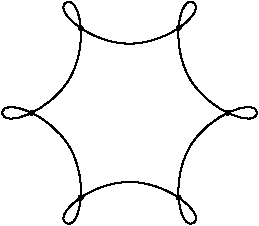
\includegraphics[height=1.1in]{main/Fig09-4A}}
\qquad
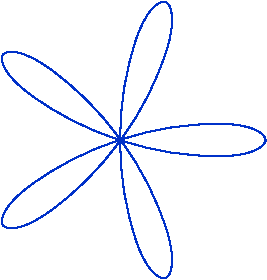
\includegraphics[height=1.2in]{main/five}
\caption{A general linear series of degree $g+2$ maps a nonhyperelliptic
curve of genus $g$
to a plane curve with $\protect\sbinom{g}{2}$ nodes
but the image of a
hyperelliptic curve has
just one singular point, where $g$ smooth branches intersect with
distinct tangents.
}
\label{Fig9.4}
\end{figure}

\begin{proof}
%\begin{itemize}
% \item (Dimension)
Since $D$ is general and $\deg D > h^{0}(K)$ we see
that $D$ is nonspecial, whence $h^0(D) = (g+2)-g+1 = 3$.
This yields the dimension claim.

%\item (no basepoints)
If $|D|$
has
a basepoint $p\in C$, then $3=h^0(D)
= h^0(D-p) = (g+1)-g+1+h^0(K_C-D+p)$,
so $K_C-D$ is effective of degree $2g-2-(g+1) =g-3$; thus the family of
such $D$ depends on only $g-3+1$ parameters,
and $\mu(D)$ would lie in a proper subvariety of $\Pic_{g+2}(C)$,
contradicting generality.

Next we show that
there are only finitely many pairs $p,
q \in C$ such that $\phi_D(p) = \phi_D(q)$; that is, $\phi_D$
is birational onto its image.
Indeed, $\phi_D(p) = \phi_D(q)$
 means that $h^0(D-p-q) = 2$. By the Riemann--Roch
 theorem, $D-p-q = K-E$ for some effective divisor $E$ of degree $g-2$;
 thus $\sO_C(D)$ is in the image of the map
$$
\nu : C_2 \times C_{g-2} \to \Pic_{g+2}(C)
$$
sending $(p+q, E)$ to $K_C - E + p + q$.
But
$\nu$ is
the composition of two surjective maps, $C_2 \times C_{g-2} \to C_g$
and $C_g\to Pic_g \to Pic_{g+2}$ by duality. Since the source and
target of $\nu$ have the same dimension, the general fiber of $\nu$ is
finite.

We turn to the types of singularities. First we eliminate tacnodes.
To say that a pair of points $p, q \in C$ map to
a point of $C_0$ such that the
two branches have a common tangent means two things: that $h^0(D-p-q)
\geq 2$; and that $h^0(D-2p-2q) \geq 1$. If this is the case, set $E =
D - 2p - 2q$.  The condition $h^0(D-2p-2q) \geq 1$ is equivalent to
$E$ being an effective divisor. Considering the canonical map $\phi_K:
C\to \PP^{g-1}$
the
geometric Riemann--Roch theorem,
\index{Riemann--Roch theorem!geometric}%
$$r(E) = \deg E -1-\dim\overlow{\phi_K(E)},$$
implies that $\overlow {\phi_K(E)}$ has
dimension $g-3$. The
further
condition $h^0(D-p-q) \geq 2$ says that
$\dim\overlow{\phi_K(E+p+q)} = g-2$,
so the secant line $\overlw20{pq}$ meets the $(g-3)$-plane
$\overlow{\phi_K(E)}$. Now, not every secant line to $C$ can meet
a given linear subspace $\Lambda \subset \PP^{g-1}$ of dimension
$g-3$\emdash otherwise, the projection $\pi_\Lambda : C \to \PP^1$ would
be constant\emdash so we see that $\mu(D)$ would have to lie on the image
of a proper subvariety of $C_{g-2} \times C_2$ under the map $(E, p+q)
\mapsto \sO(E+2p+2q)$ from $C_{g-2} \times C_2$ to $\Pic_{g+2}(C)$.
Since the dimension of this subvariety is $<g$ we see that if $C'$ has
a point at which two branches are tangent, then $\sO_C(D)$ lies in a
proper subvariety of $\Pic_{g+2}(C)$. Since
the Abel--Jacobi map $C_{g+2} \to Pic_{g+2}(C)$ is surjective,
 $D$ would not be general.

\smallbreak
Now let's suppose that $C$ is nonhyperelliptic.
To prove
claim (1) of the theorem,
we
have to show
that the image $C_0 = \phi_D(C)$
has only nodes as singularities,
rather than cusps or triple points.
That there are exactly
$\tbinom{g}{2}$ nodes then follows from the
adjunction formula.
\index{adjunction formula}%

\begin{itemize}
\item []\hskip-\leftmargini (no cusps)\,
To say that a point $p \in C$ maps to a cusp of $C_0$
(that is, the differential $d\phi_D$ is zero at $p$) amounts to saying
that $h^0(D-2p) \geq 2$; that is, $D-2p$ is a $g^1_g$. But by the
Riemann--Roch theorem, $W^1_g = K_C - W_{g-2}$; so to say $\phi_D$
has a cusp means that
$$
\mu(D) \in 2W_1 + K_C - W_{g-2},
$$
and since the locus on the right has dimension at most $g-1$, a general
point of $J(C)$ will not lie in it. Note that this subsumes the fact
that $|D|$ has no basepoints.

\item []\hskip-\leftmargini (no triple points)\,
To say that $C_0$ has a triple point means
that for some divisor $E = p+q+r$ of degree 3, $h^0(D-E) \geq 1$; thus
we must have
$$
\mu(D) \in W_3^{} + W^1_{g-1}.
$$
To argue that this is not the case, we need to know that $\dim W^1_{g-1}
\leq g-4$;
streamlined
if $C$ is nonhyperelliptic.
\end{itemize}

\noindent This concludes the proof in the nonhyperelliptic case. Now
suppose that $C$ is hyperelliptic, and let $|E|$ be the  $g^1_2$ on
$C$.
Since $D$ is a
divisor of degree $g+2$, the divisor $D - E$ will
have degree $g$, and so be effective; thus we can write
$D \sim E + p_1 + \dots + p_g$
for some
$g$ points $p_i$, which must be distinct since $D$ was assumed general.

The fact that
$$
h^0(D - p_1 - \dots - p_g) = h^0(E) = 2 = h^0(D) - 1
$$
implies that $\phi_D$ maps all the points $p_i$ to the same point. The
image curve $C_0$ thus has a point with at least $g$ branches. Since
these branches cannot share a tangent line,
they are smooth and their tangents are distinct; that is, the point is
an ordinary multiple point. By the adjunction
\index{adjunction formula}%
formula $p_a(C) = \tbinom{g+1}{2}$ and since $C$ has genus $g$ the
singularity must have $\delta$ invariant
$\tbinom{g+1}{2} -g = \tbinom{g}{2}$. Such a singularity cannot have
multiplicity $>g$, and is thus a $g$-fold point. Since the
\index{delta invariant@$\delta$ invariant}%
$\delta$ invariant of such a point is at least $\tbinom{g}{2}$ by
the discussion following Theorem~\ref{divisor classes on blowup}
(see also
Proposition~\ref{effect of blowup on genus}), the $g$-fold point is ordinary and there can be no other
singularities.
\end{proof}

\section{Exercises}

\begin{exercise}
Let $C\subset \PP^r$ be a smooth curve
over an algebraically closed field of arbitrary characteristic.
We can
re-embed $C$ by a
Veronese map,
that is, consider $\widetilde C = \nu_m(C)$ where
$\nu_m :
\PP^r \to \PP^N$ is the $m$-th Veronese map. Prove:

\begin{proposition}[%
compare
~Proposition~\ref{nodal projection}]
\label{positive characteristic nodes}
If $m$ is high enough then
the projection of~$@\widetilde C$ from a general $\PP^{N-3}$
is a birational map onto a nodal
plane curve.
\unskip\break %FMT
\null\hfill
\tohint{10.1}
\end{proposition}
\end{exercise}

\begin{npt}
\begin{exercise}[\cite{Rathmann}]
\label{strange curves} Let $k$ be an
\index{Rathmann, J\"{u}rgen}%
algebraically closed field of characteristic $p>0$, and let $q=p^e$
for some $e\geq 1$. Let $C\subset \PP^r$
be the closure of the image $C_0$ of the morphism
$$
\AA^1 \ni t \mapsto (t, t^q, t^{q^2}, \dots , t^{q^{r}}) \in \AA^r
$$
where $\AA^r\subset \PP^r$ is the open set $x_0=1$.
\begin{enumerate}
\item Show that $C$ is a complete intersection, defined by the equations
$$
x_0^{q-1}x_2 - x_1^q, x_0^{q-1}x_3 - x_2^q,\dots,
x_0^{q-1}x_r - x_{r-1}^q.
$$
\item Show that $C$ is singular unless $q = r = 2$.
\item Show every secant line to $C_0$ contains $q$ points of $C_0$;
more generally, if
$a_1, \dots, a_r$ are linearly independent points of $C_0$, show that
the linear span of
$a_1, \dots, a_r$ contains $q^{(r-1)}$ points of $C_0$.  Compare this
with the configuration of
points in affine $r$-space over a field of $q$ elements.
\end{enumerate}
\end{exercise}
\end{npt}

\begin{exercise}
Here is another approach to the $g+2$ theorem in the hyperelliptic case:
\index{g@$g+2$ theorem}%
Let $C$ be a
hyperelliptic
\index{hyperelliptic curve}%
curve of genus $g$ and $D$ a general divisor
of degree $g+1$ on $C$; let $|E|$ be the $g^1_2$ on $C$.
Consider the map $\phi : C \to \PP^1 \times \PP^1$ given as the product
of the maps $\phi_D : C \to \PP^1$ and $\phi_E : C \to \PP^1$ given by
the pencils $|D|$ and $|E|$.
\begin{enumerate}
\item Show that $\phi$ embeds the curve $C$ as a curve of bidegree
$(g+1,2)$ on $\PP^1 \times \PP^1` `$.
\item Now embed $\PP^1 \times \PP^1$ into $\PP^3$ as a quadric surface
$Q$; pick a general point $p \in C \subset Q$ and project $C$ from the
point $p$. Show that the image curve $C_0$ is a plane curve of degree
$g+2$ with one ordinary $g$-fold point.
\tohin{10.2}
\end{enumerate}\label{tnih10.2}
\end{exercise}

\begin{exercise}\label{extremal m-ics}
Establish the analogue of Proposition~\ref{rnc on most quadrics}
for hypersurfaces of any degree $m$, that is to say no irreducible,
nondegenerate curve in $\PP^d$ lies on more hypersurfaces of degree $m$
than the
rational normal curve.
\index{rational!normal curve}%
To do this, let $C\subset \PP^d$ be any irreducible nondegenerate
curve. Let $\Gamma$ be a general hyperplane section
of $C$, and use the exact sequences
$$
0 \to \cI_{C/\PP^d}(l-1) \to \cI_{C/\PP^d}(l) \to
\cI_{\Gamma/\PP^{d-1}}(l) \to 0.
$$
with $2 \leq l \leq m$ to show that
$$
h^0(\cI_{C/\PP^d}(m)) \leq  \mbinom{d+m}{m} - (md+1)
$$
with equality only~if $C$ is a rational normal curve.
\end{exercise}

\begin{exercise}\label{linear bound is sharp}
Let $D \subset \PP^r$ be a rational normal curve. If $\Gamma \subset D$
is any collection of $d$ points on $D$ (or for that matter any subscheme
of $D$ of degree $d$) then the
Hilbert function
\index{Hilbert function}%
of $\Gamma$ is
$ h_\Gamma(m) = \min\{d, mr+1\} $.
\tohint{10.5}
\end{exercise}

\begin{exercise}
Let $C$ be a reduced irreducible curve with general hyperplane section
$\Gamma$,
and write
$d-1 = M(r-1) +\epsilon$ with $\epsilon<r-1$ as in Castelnuovo's theorem.
Prove that
\begin{enumerate}
\item if $\epsilon > 0$, then $\cO_C(M)$ is nonspecial, but $\cO_C(M-1)$
is special; and
\item if $\epsilon = 0$, then $\cO_C(M-1)$ is nonspecial, but $\cO_C(M-2)$
\index{epsilon@$\epsilon=\epsilon(d,r)$}%
is special.
\tohin{10.6}
\end{enumerate}\label{tnih10.6}
\end{exercise}

\begin{exercise}\label{castelnuovo unique}
If $C \subset \PP^r$ is a
Castelnuovo curve
\index{Castelnuovo curve}%
of degree $d \geq 2r$,
show that $|D| = |\cO_C(1)|$ is the unique $g^r_d$ on $C$.
\tohint{10.7}
\end{exercise}

\begin{exercise}\label{rarity of Castelnuovo}
We have seen that complete intersections $C = Q \cap S \subset \PP^3$ of a
quadric surface $Q$ and a surface $S$ of degree $k$ achieve Castelnuovo's
bound $g = \pi(2k, 3)$ on the genus of curves of degree $2k$ in $\PP^3``$.
In fact, we will see in Chapter~\ref{ScrollsChapter} that any curve
$C \subset \PP^3$ of degree $2k$ and genus $g = \pi(2k, 3) = (k-1)^2$
is of this form.
\begin{enumerate}
\item Find the dimension of the subvariety $\Gamma \subset M_g$ consisting
of Castelnuovo curves.
\item Find the dimension of the subvariety $H \subset M_g$ of
hyperelliptic curves, and compare this to the result of the first part.
\tohin{10.8}
\end{enumerate}\label{tnih10.8}
\end{exercise}
\endgroup % redef of \mult

